% charla · creada con charlas-charlie el 2026-11-17 (estilo v1.0.0, copiado en estilo/)
% Compilar:  latexmk -pdf main.tex        Notas del orador:  latexmk -pdf -usepretex='\def\connotas{}' main.tex
% Figuras:   python make_figs.py          Decisiones de la charla: BRIEF.md
\documentclass[aspectratio=169,11pt]{beamer}
\def\tema{clasico}          % bloques | metropolis | clasico | tufte | oscuro | editorial
\def\idioma{english}      % english | spanish
\def\logos{harmonie,bsc}     % también upc; \def\logos{} sin logos
\def\fondoportada{pulmones}  % vacío | pulmones | nariz | pulmones-original | malla | remolinos | figs/mi-fondo.png
\def\progreso{numeros}       % numeros | barra | ambos
\makeatletter\def\input@path{{estilo/}}\makeatother
\input{preambulo}

\title{Newton beats Picard\\ on strongly nonlinear diffusion}
\subtitle{Residual convergence on a 1D model problem}
\author{Carlos Arnedo Joya}
\institute{Barcelona Supercomputing Center}
\date{\today}

\begin{document}

\begin{frame}[plain]
  \titlepage
\end{frame}

%======================================================================
\begin{frame}{A $u$-dependent diffusivity forces us to iterate}
  \noindent
  \begin{columns}[c,onlytextwidth]
    \begin{column}{0.48\textwidth}
      \[ -\big(k(u)\,u'\big)' = f, \quad u(0)=u(1)=0 \]
      \[ k(u) = k_0 + u^2, \quad f = 20 \]
      \begin{itemize}\setlength\itemsep{0.7em}
        \item The matrix depends on $u$: \alert{iterate}.
        \item Smaller $k_0$: stronger nonlinearity.
      \end{itemize}
      \vspace{0.4cm}
      {\footnotesize\color{tenue}Finite differences, 199 nodes, synthetic data.}
    \end{column}
    \begin{column}{0.48\textwidth}
      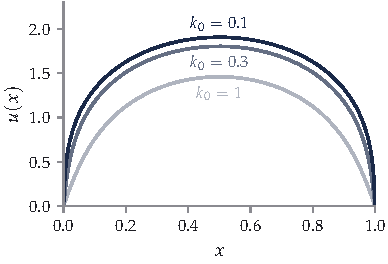
\includegraphics{figs/perfiles.pdf}
    \end{column}
  \end{columns}
  \note{Model problem: 1D steady nonlinear diffusion, porous-medium-like diffusivity. k0 controls how
    nonlinear the problem is: with k0 = 0.1 and u around 1.9, k changes by a factor ~37 across the domain.
    All the data in the talk comes from make\_figs.py (FD, 199 interior nodes).}
\end{frame}

%======================================================================
\begin{frame}{Both methods share the loop; only step 2 differs}
  \vspace{0.5cm}
  \centering
  %% Nonlinear iteration loop shared by Picard and Newton (from the charlas-charlie template flujo.tex).
%% Steps 1 and 3 are common (serieC); step 2, where the methods differ, in serieB.
%% Picard in serieA and Newton in serieD, the same colours as in figs/convergencia.pdf.
\begin{tikzpicture}[
    caja/.style={fill=#1!12!fondo,draw=tinta,line width=0.6pt,rounded corners=3pt,align=left,inner sep=5pt,
      font=\scriptsize,text width=2.7cm,minimum height=2.9cm},
    sol/.style={fill=#1,text=white,rounded corners=1.5pt,inner sep=1.4pt,font=\tiny\bfseries,
      minimum height=0pt,minimum width=0pt,text width={},align=center},   % TikZ anidado: resetear
    flecha/.style={-{Stealth[length=5pt]},tinta,line width=0.8pt}]
  \newcommand\etiqueta[2]{\tikz[baseline=(c.base)]\node[sol=#1](c){#2};}
  \node[caja=serieC] (a) at (0,0)
    {\textbf{1 · Residual}\\[3pt] $R(u^k) = A(u^k)\,u^k - f$\\[3pt] {\color{tenue}same for both}};
  \node[caja=serieB,right=0.45cm of a,text width=3.9cm] (b)
    {\textbf{2 · Linearize and solve}\\[5pt]
     {\color{serieA}\textbf{Picard}} \etiqueta{serieA}{CG}\\[1pt] $A(u^k)\,u^{k+1} = f$\\
     {\color{tenue}symmetric, $k$ frozen}\\[5pt]
     {\color{serieD}\textbf{Newton}} \etiqueta{serieD}{GMRES}\\[1pt] $J(u^k)\,\delta u = -R(u^k)$\\
     {\color{tenue}non-symmetric, with $k'(u)$}};
  \node[caja=serieC,right=0.45cm of b] (c)
    {\textbf{3 · Update}\\[3pt] $u^{k+1} = u^k + \delta u$\\[3pt] {\color{tenue}Picard: $u^{k+1}$ directly}};
  \draw[flecha] (a) -- (b); \draw[flecha] (b) -- (c);
  \begin{scope}[on background layer]
    \node[fill=tinta!4!fondo,rounded corners=5pt,inner xsep=8pt,inner ysep=10pt,fit=(a)(b)(c)] (it) {};
  \end{scope}
  \node[anchor=south west,font=\scriptsize\bfseries,inner sep=1pt] at ($(it.north west)+(0.15,0.02)$)
    {Nonlinear iteration $k \to k{+}1$};
  \draw[flecha,acento] (c.south) -- ++(0,-0.62) -| node[pos=0.25,below,font=\scriptsize,text=tinta]
    {$\|R(u^{k+1})\| / \|R(u^0)\| > 10^{-8}$? \ iterate again} (a.south);
  \draw[flecha] ($(it.west)+(-0.55,0)$) node[left,font=\small]{$u^0$} -- (it.west);
  \draw[flecha] (it.east) -- ++(0.45,0) node[right,font=\small]{$u$};
\end{tikzpicture}

  \note{Same three steps. Picard freezes k at the previous iterate and solves a symmetric system for
    u directly. Newton also differentiates k, which gives a non-symmetric Jacobian and a correction
    delta u. Both start from the linear solution (k = 1) and stop at a relative residual of 1e-8.}
\end{frame}

%======================================================================
\begin{frame}{Picard converges linearly, Newton quadratically}
  \noindent
  \begin{columns}[T,onlytextwidth]
    \begin{column}{0.48\textwidth}
      {\color{serieA}\textbf{Picard}: linear convergence}
      \[ \|e^{k+1}\| \approx \rho\,\|e^{k}\| \]
      \begin{itemize}\setlength\itemsep{0.6em}
        \item $\rho$ grows with the nonlinearity.
        \item $\rho \ge 1$: no convergence.
      \end{itemize}
    \end{column}
    \begin{column}{0.48\textwidth}
      {\color{serieD}\textbf{Newton}: quadratic convergence}
      \[ \|e^{k+1}\| \le C\,\|e^{k}\|^2 \]
      \begin{itemize}\setlength\itemsep{0.6em}
        \item Close: $10^{-2} \to 10^{-4} \to 10^{-8}$.
        \item Far: no guarantee.
      \end{itemize}
    \end{column}
  \end{columns}
  \vspace{0.6cm}
  \mensaje{Prediction: as $k_0$ drops, Picard slows down; Newton does not.}
  \note{The theory in one slide. Picard is a fixed-point iteration: its contraction factor depends on
    how strongly k depends on u. Newton is quadratic in a neighbourhood of the solution.}
\end{frame}

%======================================================================
\begin{frame}{Newton: 5--7 iterations; Picard: 11--33, then it stalls}
  \vspace{0.3cm}
  \noindent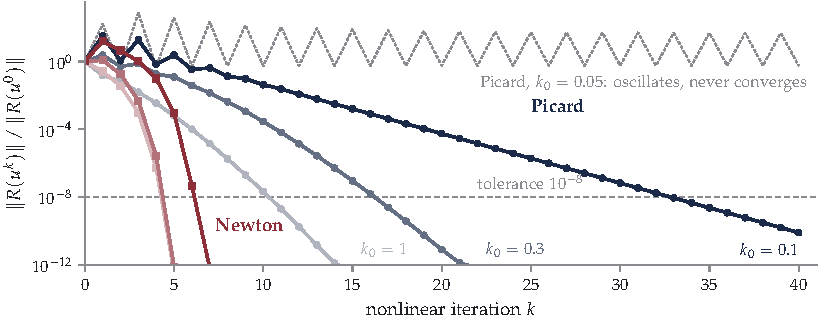
\includegraphics{figs/convergencia.pdf}
  \note{Residual history, relative to the initial residual. Lighter = milder nonlinearity. Newton:
    the last two or three iterations drop by many orders of magnitude (quadratic). Picard: straight lines
    on the log scale (linear), with a slope that flattens as k0 drops; at k0 = 0.05 it oscillates and
    never converges without relaxation.}
\end{frame}

%======================================================================
\begin{frame}{Newton still wins with a step $2\times$ as expensive}
  \noindent
  \begin{columns}[c,onlytextwidth]
    \begin{column}{0.55\textwidth}
      \begin{tabular}{@{}lccc@{}}
        \toprule
        {\color{tenue}$k_0$} & {\color{tenue}Picard} & {\color{tenue}Newton} & {\color{tenue}break-even} \\
        \midrule
        $1$    & 11 & 5 & $2.2\times$ \\
        $0.3$  & 17 & 5 & $3.4\times$ \\
        $0.1$  & 33 & 7 & $4.7\times$ \\
        $0.05$ & \alert{stalls} & 8 & $\infty$ \\
        \bottomrule
      \end{tabular}\par\vspace{0.25cm}
      {\footnotesize\color{tenue}Iterations to $10^{-8}$. Break-even: Newton/Picard cost per step at
      which both take the same time.}
    \end{column}
    \begin{column}{0.4\textwidth}
      \begin{itemize}\setlength\itemsep{0.8em}
        \item A Newton step: $k'(u)$ and GMRES instead of CG.
        \item Typically $1.5$--$2\times$ a Picard step.
      \end{itemize}
    \end{column}
  \end{columns}
  \note{Iteration counts are from the model problem. The 1.5-2x per-step cost is a typical figure for
    GMRES vs CG with the same preconditioner, not measured here (1D, direct solver).}
\end{frame}

%======================================================================
\begin{frame}{Use Newton when $k$ varies strongly with $u$}
  \vspace{0.4cm}
  \begin{enumerate}\setlength\itemsep{1.1em}
    \item Same loop, different matrix: Newton adds $k'(u)$ and loses symmetry.
    \item Picard slows down as the nonlinearity grows, then stalls;
          Newton stays at \alert{5--8 iterations}.
    \item Newton pays off whenever its step costs less than $2\times$ a Picard step.
  \end{enumerate}
  \vspace{0.6cm}
  {\color{tenue}Next: Picard to get close, then Newton; a line search for poor starts.}
  \note{Three messages. The hybrid Picard-then-Newton strategy addresses Newton's need for a good
    initial guess.}
\end{frame}

\end{document}
